\documentclass[conference]{IEEEtran}
\IEEEoverridecommandlockouts
\usepackage{cite}
\usepackage{amsmath,amssymb,amsfonts}
\usepackage{algorithmic}
\usepackage{graphicx}
\usepackage{textcomp}
\usepackage{xcolor}
\usepackage{booktabs}
\usepackage{multirow}
\usepackage{array}
\usepackage{url}

\def\BibTeX{{\rm B\kern-.05em{\sc i\kern-.025em b}\kern-.08em
    T\kern-.1667em\lower.7ex\hbox{E}\kern-.125emX}}

\begin{document}

\title{TAIRO: Trustworthiness Evaluation of Robotic Policies
Under Adversarial Cyberattacks}


\author{
\IEEEauthorblockN{Yves Velasquez Vega}
\IEEEauthorblockA{
\textit{California State University, Fullerton}\\
Fullerton, California\\
vyves@csu.fullerton.edu}
\and
\IEEEauthorblockN{Jachin Choi}
\IEEEauthorblockA{
\textit{Case Western Reserve University}\\
Cleveland, Ohio\\
jmc440@case.edu}
\and
\IEEEauthorblockN{Sunny Sood}
\IEEEauthorblockA{
\textit{University of Missouri-Kansas City}\\
Kansas City, Missouri\\
sks6nv@umkc.edu}
\and
\IEEEauthorblockN{Abhinav Kochar}
\IEEEauthorblockA{
\textit{University of Missouri-Kansas City}\\
Kansas City, Missouri\\
arkrnr@umkc.edu}
\and
\IEEEauthorblockN{Duy Ho}
\IEEEauthorblockA{
\textit{Department of Computer Science}\\
\textit{California State University, Fullerton}\\
Fullerton, California\\
duyho@fullerton.edu}
\and
\IEEEauthorblockN{Yugyung Lee}
\IEEEauthorblockA{
\textit{University of Missouri-Kansas City}\\
Kansas City, Missouri\\
leeyu@umkc.edu}
}



\maketitle

\begin{abstract}
Robotics cybersecurity surveys catalog vulnerabilities and attack classes and recommend system-design countermeasures such as authentication and cryptographic protection, but do not quantify how a learned control policy's task performance degrades under attack. Robust-RL benchmarks address this empirically, but frame perturbations as generic statistical or adversarial noise rather than cybersecurity-specific threat models, and do not evaluate online failure detection, recovery, or a principled trustworthiness score.
TAIRO addresses this gap on the
contact-rich, sparse-reward FetchPickAndPlace-v4 manipulation task, evaluating a
Soft Actor-Critic with Hindsight Experience Replay (SAC+HER) policy under an
eleven-condition cybersecurity attack taxonomy spanning observation-, goal-, and
action-space perturbations (including three manipulation-specific attacks targeting
object pose and gripper state), a classifier-conditioned adaptive recovery controller
that blends specialized feature-based recovery experts online according to a failure-mode
classifier, and a five-component composite trustworthiness score grounded in the NIST AI
Risk Management Framework. We
show that policy vulnerability is strongly dependent on the attack surface: SAC+HER
maintains high success under several action-space attacks but degrades substantially
under sensor and goal-channel corruption. Recovery-aware control is validated in a
FetchReach-v4 pilot using a threshold-based fallback controller, and extended to
FetchPickAndPlace-v4 with a classifier-conditioned adaptive recovery controller (CCAR)
evaluated on the clean-trained 2M policy, where it recovers only the action-timing
attacks and leaves observation and goal-channel damage largely unrecovered, a limit we
trace to the online classifier's early-episode reliability. We additionally report a
scoped negative result: domain-randomized training failed to learn the grasp phase at
the 500k budget and recovered it only partially at 2M (44.7\% clean success, still far
below the clean-trained policy's 100\%), underscoring that robustness-oriented training
strategies must preserve sufficient clean-task signal to acquire the base skill they are
meant to protect. These findings
establish a principled vocabulary for policy-dependent attack-surface analysis and
provide a path toward higher-fidelity simulation environments, including Habitat and
Isaac Sim.
\end{abstract}



\begin{IEEEkeywords}
adversarial robustness, reinforcement learning, robot manipulation, SAC+HER,
cybersecurity, trustworthiness, NIST RMF, failure recovery, FetchPickAndPlace
\end{IEEEkeywords}


% =============================================================================
\section{Introduction}
% =============================================================================

The deployment of learned robot policies in physical environments introduces security
concerns that differ from classical software vulnerabilities and static adversarial
examples. A robot policy trained with reinforcement learning (RL) continuously maps
sensor observations to control actions, making both the observation channel and the
action channel potential attack surfaces. In embodied AI and robotic systems, attacks
may arise from corrupted sensors, spoofed goals, compromised communication links,
malicious command injection, or actuator-level manipulation~\cite{xing2025robustembodied}.
Unlike image-classification attacks, adversarial attacks on RL policies unfold over
time: an isolated corrupted observation may be recoverable, whereas sustained action
reversal or sensor dropout can accumulate across a trajectory and lead to task failure.
Prior work has shown that neural-network policies are vulnerable to adversarial
perturbations~\cite{huang2017adversarial} and that adversarial attacks can substantially
degrade deep RL performance~\cite{pattanaik2018robust}.

Recent benchmarks such as Robust-Gymnasium provide an important step toward systematic
evaluation of robust RL by supporting disruptions across observations, actions, rewards,
and environments~\cite{gu2025robustgymnasium}. However, existing benchmarks primarily
measure performance degradation under perturbation. They do not fully address three
questions that are critical for trustworthy robotics: (i) whether the system can detect
and recover from attack-induced failures online, (ii) whether robustness should be
scored using a broader trustworthiness framework rather than success rate alone, and
(iii) how the relationship between attack surface and policy architecture determines
failure modes. These gaps are especially important for robotic manipulation, where
sparse rewards, contact-rich dynamics, and closed-loop control can make failures abrupt,
difficult to diagnose, and safety-relevant.

We introduce TAIRO (Trustworthy AI Robotics), a failure-aware evaluation framework for
assessing robotic control policies under adversarial cybersecurity perturbations. TAIRO
uses Soft Actor-Critic (SAC), a maximum-entropy off-policy RL algorithm for continuous
control~\cite{haarnoja2018soft}, together with Hindsight Experience Replay (HER), which
is designed for sparse and binary reward settings in robotic manipulation~\cite{andrychowicz2017hindsight}.
We evaluate the framework on the FetchPickAndPlace-v4 manipulation task from
Gymnasium-Robotics, where a Fetch manipulator must grasp a free-floating object and move
it to a target position in Cartesian space~\cite{gymnasiumrobotics2024,fetchreachdoc}.
The framework was first validated on the lower-dimensional FetchReach-v4 reaching task;
this pilot study is summarized in Appendix~\ref{app:fetchreach}. To connect empirical
robustness results to AI risk governance, TAIRO defines a five-component trustworthiness
score grounded in the NIST AI Risk Management Framework~\cite{nist2023airmf}.

TAIRO's central contribution is not simply training a policy under attack, but
benchmarking how different cyber-physical attacks degrade a manipulation policy and
using failure detection together with recovery-aware control to decide when and how
the robot should recover. Concretely, TAIRO makes the following contributions:

\begin{itemize}
    \item An eleven-condition cybersecurity attack taxonomy covering observation-space
          perturbations (sensor dropout, sensor bias), goal-space perturbations
          (immediate and mid-episode goal spoofing), action-space perturbations
          (clipping, delay, and reversal), and three manipulation-specific attacks
          targeting object pose, gripper actuation, and contact sensing, used to
          systematically benchmark how each attack degrades a sparse-reward,
          contact-rich manipulation policy.

    \item A failure-aware recovery system evaluated in two forms: a threshold-based
          fallback controller validated in the FetchReach-v4 pilot, and a
          classifier-conditioned adaptive recovery controller (CCAR) for
          FetchPickAndPlace-v4 that softly blends specialized feature-based recovery
          experts according to an online failure-mode classifier, evaluating recovery
          effectiveness using outcome-referenced metrics rather than trigger frequency
          alone.

    \item An empirical evaluation of SAC+HER on the sparse-reward, contact-rich
          FetchPickAndPlace-v4 manipulation task, building on a validated pilot study
          on FetchReach-v4 that demonstrated HER is load-bearing for non-zero task
          success in sparse-reward settings.

    \item A five-component trustworthiness scoring methodology that moves beyond
          raw success rate by accounting for reliability, robustness, cyber resilience,
          safety, and recovery.

    \item A scoped negative result on domain-randomized training, showing that
          exposing a policy to attack conditions during training can prevent it from
          acquiring the base grasping skill at a small budget and recover it only
          partially at a larger one.

    \item A migration roadmap from FetchPickAndPlace-v4 to higher-fidelity manipulation
          and embodied-AI simulation environments, including Habitat-based home
          simulation~\cite{puig2023habitat3} and Isaac Sim for scalable, high-fidelity
          robotics simulation~\cite{nvidia2026isaacsim}.
\end{itemize}

The remainder of this paper is organized as follows. Section~\ref{sec:related} reviews
related work on adversarial RL, embodied-AI security, and robot robustness. Section~\ref{sec:method}
describes the TAIRO framework, attack taxonomy, and recovery system. Section~\ref{sec:eval}
presents the evaluation protocol and trustworthiness scoring methodology. Section~\ref{sec:results}
reports FetchPickAndPlace-v4 results. Section~\ref{sec:discussion} discusses
findings, limitations, and the fidelity gap. Section~\ref{sec:conclusion} concludes
with the planned migration roadmap. Appendix~\ref{app:fetchreach} summarizes the
FetchReach-v4 pilot study that preceded and shaped this work.

% =============================================================================
\section{Related Work}
\label{sec:related}
% =============================================================================

\subsection{Adversarial Attacks on RL Policies}

Huang et al.~\cite{huang2017adversarial} showed that trained deep reinforcement
learning (RL) policies are vulnerable to adversarial perturbations applied to
observations, including fast gradient sign method (FGSM)-style attacks. Their results
demonstrated substantial performance degradation across Atari and MuJoCo tasks,
establishing that strong clean-task performance does not imply robustness. Pattanaik
et al.~\cite{pattanaik2018robust} extended this line of work to robust deep RL under
adversarial attacks, showing that small perturbations to policy inputs can cause severe
degradation in continuous-control settings.

These studies motivate systematic evaluation of RL policies under controlled attacks.
However, much of the adversarial RL literature focuses primarily on observation-space
perturbations. In deployed robotic systems, the attack surface is broader: adversaries
may corrupt sensor readings, spoof goals, delay or clip actuator commands, reverse
actions, or interfere with communication between perception, planning, and actuation
modules. TAIRO therefore evaluates observation-space, action-space, and goal-space
attacks within a unified robotics-oriented cybersecurity framework.

\subsection{Robustness Benchmarks for Robot Policies}

Robust-Gymnasium~\cite{gu2025robustgymnasium} introduced a modular benchmark for
evaluating RL policy robustness under diverse perturbations, including observation
disruptions, action disruptions, reward disruptions, and environment changes. This work
provides the closest benchmark-level comparison for TAIRO because it supports systematic
stress testing of RL agents under multiple perturbation channels.

RRLS, the Robust Reinforcement Learning Suite~\cite{zouitine2024rrls}, benchmarks robust
RL agents under uncertain or shifted MuJoCo dynamics. TAIRO differs in framing
perturbations as cybersecurity-relevant compromises of sensor buses, actuator command
channels, stale command replay, or mission targets rather than as dynamics mismatch.

TAIRO builds on these robustness benchmarks but differs in four main ways. First, it
focuses on sparse-reward, contact-rich robotic manipulation, where SAC+HER is necessary
for reliable task success. Second, it frames each perturbation as a cybersecurity-relevant
threat model rather than only as generic robustness noise, including three attacks
specific to object grasping and manipulation that have no analogue in existing
observation/action disruptor taxonomies. Third, it introduces a multi-component
trustworthiness score rather than relying only on task success or robustness
degradation. Fourth, it evaluates online recovery behavior during episode execution.

\subsection{Cybersecurity-Oriented Attack Surfaces in Embodied AI}

Recent embodied-AI security surveys~\cite{xing2025robustembodied} emphasize that
robotic and embodied agents are vulnerable across the perception, planning, and
actuation stack. These surveys identify sensor compromise, goal manipulation,
communication interference, and actuator-level attacks as important threat vectors.
TAIRO operationalizes these concerns through an explicit attack taxonomy.

The observation-space attacks in TAIRO include sensor dropout, which simulates complete
loss of sensor fields, and sensor bias, which simulates systematic tampering through a
fixed offset. The action-space attacks include clipping, delay, and reversal,
corresponding to actuator saturation, stale command replay, and complete hijacking of
the action command channel. The goal-space attacks include immediate goal spoofing and
mid-episode goal spoofing, where a false target is injected either at mission start or
after the robot has already begun execution. The manipulation-specific attacks target
object-tracking and gripper-actuation channels that are only present once the task
requires grasping and transporting an object, extending the taxonomy beyond what a
pure end-effector-positioning task can expose. Together, these attack conditions provide
a more cybersecurity-oriented evaluation protocol than generic noise injection alone.

\subsection{Hindsight Experience Replay for Sparse-Reward Robotics}

Hindsight Experience Replay (HER) was introduced by Andrychowicz et
al.~\cite{andrychowicz2017hindsight} to address sparse and binary reward problems in
goal-conditioned reinforcement learning. HER relabels failed trajectories using goals
that were actually achieved, thereby providing useful learning signal even when the
original goal was not reached. This mechanism is especially important for robotic
manipulation tasks, where random exploration rarely produces successful outcomes.

In TAIRO, HER is not simply a performance enhancement; it is a load-bearing component of
the evaluation pipeline. Our FetchReach-v4 pilot study (Appendix~\ref{app:fetchreach})
shows that plain SAC~\cite{haarnoja2018soft} achieves near-zero success under sparse
rewards, while SAC+HER achieves reliable clean-task success. This distinction is
important because robustness evaluation is meaningful only when the base policy first
solves the nominal task, and it motivated using SAC+HER as the sole learned policy for
the more expensive FetchPickAndPlace-v4 evaluation.

\subsection{Recovery-Aware Control and Failure Detection}

Most adversarial RL benchmarks quantify how much performance degrades under attack, but
they do not typically evaluate whether the robot can detect failure conditions and
recover during execution. TAIRO addresses this gap through an iteratively refined
recovery mechanism. The initial recovery logic used action magnitude and increasing
distance to the goal as failure indicators, but it produced false positives on clean
episodes and was insufficient for several attack modes. The improved detector monitors
sustained action-norm saturation and progress toward the goal, reducing clean-trigger
false positives while enabling more effective recovery under sensor dropout.

The final recovery design holds a rule-based fallback controller for multiple steps
after a trigger rather than applying only a single corrective action. This design is
important because some attacks require sustained corrective behavior. As discussed in
Section~\ref{sec:discussion}, not all attacks are equally recoverable, and the detector
originally calibrated on FetchReach-v4 requires re-examination on FetchPickAndPlace-v4,
where the action space is four-dimensional rather than three-dimensional.

\subsection{Trustworthiness Frameworks for AI Systems}

The NIST AI Risk Management Framework~\cite{nist2023airmf} provides a structured
vocabulary for evaluating AI systems along trustworthiness dimensions such as validity,
reliability, safety, security, robustness, resilience, accountability, and transparency.
TAIRO adapts this risk-management perspective to the RL policy evaluation setting by
mapping rollout-level measurements to quantitative trustworthiness sub-scores.

Unlike qualitative or human-audit-based trustworthiness assessments, TAIRO computes
trustworthiness scores directly from logged episode trajectories. The proposed scoring
framework combines reliability, robustness, cyber resilience, safety, and recovery.
This makes the evaluation reproducible and enables comparison across attack conditions,
policy architectures, and recovery strategies. In this way, TAIRO connects adversarial
RL benchmarking with broader AI risk-management principles.


% =============================================================================
\section{Method}
\label{sec:method}
% =============================================================================

\subsection{TAIRO Framework Overview}

TAIRO evaluates the trustworthiness of robotic control policies under
cybersecurity-relevant adversarial perturbations. The framework consists of four
integrated components: (1) a simulation environment with pluggable attack wrappers,
(2) the SAC+HER learned policy under evaluation, with a rule-based controller used
internally by the recovery module rather than benchmarked as a standalone policy,
(3) an online recovery controller that intervenes when attack signatures
are detected, and (4) a recovery-aware trustworthiness scoring module that summarizes
episode-level behavior into interpretable sub-scores and a composite score.

\begin{figure}[htbp]
\centerline{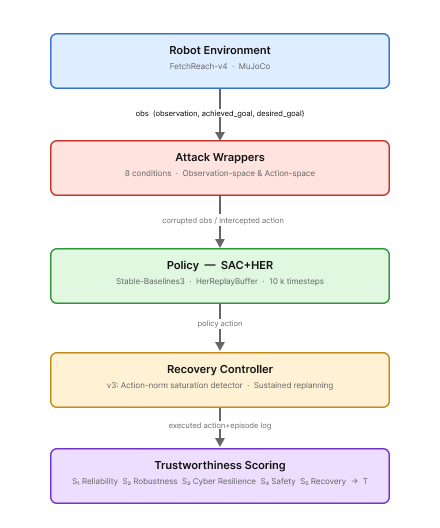
\includegraphics[width=\columnwidth]{paper_figures/tairo_framework_diagram.png}}
\caption{Overview of the TAIRO framework. Attack wrappers perturb the observation,
goal, or action channels during policy execution. The recovery controller monitors
action magnitude and progress toward the goal, then temporarily substitutes a
rule-based fallback controller when attack-like behavior is detected.}
\label{fig:framework}
\end{figure}

The central idea is to evaluate not only whether a policy succeeds under attack, but
also how it fails, whether the failure is detectable, and whether the system can recover
during execution. This recovery-aware perspective distinguishes TAIRO from robustness
benchmarks that report only task-performance degradation.

\subsection{From FetchReach-v4 to FetchPickAndPlace-v4}

We initially validated the TAIRO framework, including the attack taxonomy, recovery
controller, and trustworthiness scoring methodology, on FetchReach-v4, a
lower-dimensional reaching task from Gymnasium-Robotics. This pilot study confirmed
that Hindsight Experience Replay is load-bearing for sparse-reward success in this
setting and established the three-iteration recovery controller design described
below. A condensed summary of the FetchReach-v4 pilot results is provided in
Appendix~\ref{app:fetchreach}. We then scaled the framework to FetchPickAndPlace-v4, a
substantially harder contact-rich manipulation task requiring grasping and transport
rather than pure end-effector positioning, which is the focus of the remainder of this
paper. The transition required extending the episode budget, re-deriving attack
semantics for object-relative observations, and introducing three manipulation-specific
attacks, described in Section~\ref{sec:attacks}.

\subsection{Simulation Environment}

We use FetchPickAndPlace-v4 from Gymnasium-Robotics~\cite{gymnasiumrobotics2024}, a
goal-conditioned robotic manipulation task implemented in MuJoCo. The task requires a
Fetch robot arm to grasp a free-floating object and move it to a randomly sampled
three-dimensional target position, which may be on the table surface or in the air. An
episode is successful when the final distance between the object and the target is less
than or equal to 0.05~m. Each episode is capped at 150 steps.

The environment observation is represented as a dictionary with three fields:
\texttt{observation}, \texttt{achieved\_goal}, and \texttt{desired\_goal}. The
\texttt{observation} field is a 25-dimensional vector containing the end-effector
position and velocity, the object's position, rotation, and linear/angular velocity
relative to the gripper, and the gripper's own state and finger width. The
\texttt{achieved\_goal} field contains the current object position, since the object,
not the end effector, must reach the target, and the \texttt{desired\_goal} field
contains the target position. Rewards are sparse and binary: the agent receives $-1$ at
each non-successful step and $0$ upon success.

FetchPickAndPlace-v4 is a substantially harder task than FetchReach-v4. Success
requires not only reaching a target but grasping and stably transporting an object,
introducing a contact-rich, multi-phase control problem (approach, grasp, lift,
transport, release) that is not present in pure reaching. This motivates a larger
observation space, a longer episode budget, and re-examination of attack semantics on
object-position and goal observations relative to our earlier FetchReach-v4 pilot.

\subsection{Policy Implementations}

The benchmarked policy on FetchPickAndPlace-v4 is SAC+HER. A rule-based proportional
controller, operating on goal-space and object-relative information rather than the full
proprioceptive observation vector, is used internally by the recovery module as a
fallback expert; it is not benchmarked as a standalone policy in this study. A
uniform-random policy is retained only as a conceptual lower bound and is likewise not
reported here.

\textbf{SAC+HER:} The primary learned policy combines SAC~\cite{haarnoja2018soft} with
Hindsight Experience Replay (HER)~\cite{andrychowicz2017hindsight}, implemented using
the Stable-Baselines3 HER replay buffer~\cite{sb3}. We use future-goal relabeling with
$n_{\mathrm{sampled\_goal}}=4$, $\gamma=0.95$, and $\tau=0.05$. We evaluate SAC+HER
checkpoints trained under clean conditions at 500k and 2M timesteps, and, as a
robustness-training ablation, checkpoints trained under an attack-randomization curriculum
at the same two budgets (Section~\ref{sec:randomized_ablation}). Under clean conditions,
the clean-trained SAC+HER policy achieves reliable task success and therefore serves as
the main policy for attack and recovery evaluation. The plain-SAC-without-HER ablation
establishing the necessity of HER was conducted during the FetchReach-v4 pilot
(Appendix~\ref{app:fetchreach}) and was not repeated on FetchPickAndPlace-v4.

\subsection{Cybersecurity Attack Taxonomy}
\label{sec:attacks}

TAIRO implements a cybersecurity-oriented attack taxonomy across three channels:
observation space, goal space, and action space. Each attack is implemented as an
environment wrapper that modifies either the policy-visible observation, the
policy-visible goal, or the executed action. Eight attacks generalize directly from
our FetchReach-v4 pilot taxonomy; three additional attacks are introduced specifically
for the object-manipulation setting.

\subsubsection{Observation-Space Attacks}

\textbf{Sensor Dropout:} The policy-visible \texttt{observation} vector is replaced
with zeros at every step. This simulates denial-of-service on the sensor bus, sensor
firmware failure, or loss of proprioceptive and object-tracking state.

\textbf{Sensor Bias:} A fixed offset vector sampled once per episode from
$\mathcal{U}(-0.10,+0.10)^d$ is added to the policy-visible \texttt{observation}
field at every step. This simulates systematic sensor tampering or man-in-the-middle
manipulation. This magnitude was matched by construction to the goal-spoofing offset
scale used elsewhere in the taxonomy rather than independently derived from
FetchPickAndPlace-v4 observation statistics; we flag this as a limitation
(Section~\ref{sec:discussion}) and leave an empirical magnitude sweep to future work.

\subsubsection{Goal-Space Attacks}

\textbf{Immediate Goal Spoofing:} A random three-dimensional offset sampled from
$\mathcal{U}(-0.10,+0.10)^3$ is added to the policy-visible
\texttt{desired\_goal} from the beginning of the episode.

\textbf{Mid-Episode Goal Spoofing:} The same goal offset is injected after step 60 of
the 150-step episode, preserving the same relative onset timing (40\% of the episode
budget) used in our FetchReach-v4 pilot. This tests whether a robot that has already
begun transporting the object toward the correct goal can be redirected by a delayed
command-injection attack.

\subsubsection{Action-Space Attacks}

\textbf{Action Clipping:} Each executed action component is clipped to
$[-0.30,+0.30]$, reducing the effective actuation range.

\textbf{Action Delay:} The environment executes the previous policy action rather than
the current one, simulating network latency injection or command-buffer manipulation.

\textbf{Action Reversal:} The executed action is the negation of the policy action,
$a_{\mathrm{exec}} = -a_{\mathrm{policy}}$, simulating full command-channel hijack.

\subsubsection{Manipulation-Specific Attacks}

The transition from FetchReach-v4 to FetchPickAndPlace-v4 introduces object-relative
state and a discrete gripper actuator that are absent from the pure-reaching task. We
introduce three attacks that specifically target this new attack surface.

\textbf{Object Pose Spoofing:} The object-position sub-vector of the policy-visible
observation (\texttt{obs[3:6]}) is corrupted, independent of the rest of the
observation. This simulates a compromised object-tracking or vision subsystem while
leaving proprioceptive and goal information intact, isolating the effect of corrupted
object-relative state from general sensor failure.

\textbf{Grip State Falsification:} Only the gripper-actuation component of the
executed action (\texttt{action[3]}) is corrupted; the three end-effector displacement
components are executed as issued. This simulates compromise of the gripper control
channel specifically, such as a spoofed grasp/release command, and tests whether
transport-phase control remains viable when only grasp integrity is attacked.

\textbf{Contact Dropout:} The object-relative position, rotation, and velocity fields
of the observation (\texttt{obs[3:9]} and \texttt{obs[11:20]}) are zeroed, while the
gripper finger-width fields (\texttt{obs[9:11]}) are preserved. This simulates loss of
object-tracking or contact-sensing while leaving basic gripper-state feedback intact,
distinguishing loss of object awareness from complete sensor dropout.

These three attacks are correctly scoped to the 25-dimensional FetchPickAndPlace-v4
observation and action layout and have no analogue in the FetchReach-v4 taxonomy, since
that task involves neither object manipulation nor a load-bearing gripper actuator.

\subsection{Recovery Controller}

The TAIRO recovery controller intervenes online when the policy exhibits attack-like
behavior. The threshold-based design was developed and validated through three iterations
during the FetchReach-v4 pilot study (Appendix~\ref{app:fetchreach}), each addressing a
failure mode observed in the previous version. For FetchPickAndPlace-v4, rather than
re-tune a single action-norm threshold for a larger and more heterogeneous attack
surface, we replace fixed-threshold detection with a classifier-conditioned adaptive
recovery controller (Recovery v4, CCAR) that blends specialized feature-based recovery
experts according to an online failure-mode classifier. We summarize the v1--v3 pilot
lineage below and then describe Recovery v4, whose FetchPickAndPlace-v4 results appear in
Section~\ref{sec:results}.

\subsubsection{Recovery v1: Baseline Detector}

The initial detector used step-to-step action divergence and increasing distance from
the goal as failure indicators. Specifically, it monitored
$\lVert a_t-a_{t-1}\rVert$ and a short-horizon distance trend. However, healthy
SAC+HER policies often produce large action changes during the initial convergence
phase. As a result, v1 triggered recovery on clean episodes and effectively replaced
the learned policy with the rule-based controller even when no attack was present. This
made v1 unsuitable for trustworthiness evaluation because it could not distinguish
true recovery from clean false positives.

\subsubsection{Recovery v2: Calibrated Detector}

Recovery v2 replaces action divergence with action-norm saturation. The detector fires
when
\[
\lVert a_t\rVert > \tau_{\mathrm{sat}}
\]
for three consecutive steps. This captures a common attack signature: under severe
perturbation, the learned policy continues to produce large actions rather than
gradually reducing action magnitude as it approaches the goal. The threshold
$\tau_{\mathrm{sat}}$ was originally calibrated at $1.8$ for FetchReach-v4's
three-dimensional action space (Appendix~\ref{app:fetchreach}). Because Recovery v4
(below) replaces this fixed threshold on PickAndPlace, $\tau_{\mathrm{sat}}$ is not
re-tuned for that task; we report the underlying diagnostic for reference. Clean-condition PickAndPlace action
norms (clean\_2M, 22{,}500 steps) have $p_{50}=0.981$, $p_{95}=1.557$, $p_{99}=1.851$,
and a maximum of $1.973$. The existing threshold of $1.8$ sits above the clean $p_{95}$
(1.8 $>$ 1.557), but 1.73\% of individual clean steps already exceed it, a materially
larger tail than the FetchReach-v4 regime this threshold was originally calibrated on.
Whether this tail causes false triggers depends on whether high-norm steps cluster
consecutively, which is unresolved and left for the classifier-driven redesign to
address directly rather than via further threshold tuning.

v2 also includes a distance-progress condition to detect cases in which the robot keeps
moving away from the goal. To reduce false positives near the target, this condition is
activated only when the distance exceeds a minimum floor. This calibration eliminates
clean-episode false positives and improves recovery under sensor dropout, where the
learned policy becomes unreliable but the rule-based fallback can still guide motion
using goal-space information.

\subsubsection{Recovery v3: Sustained Recovery}

Recovery v2 applies only short corrective interventions. Under severe attacks, control
may return immediately to the attacked learned policy, producing an oscillation in which
the fallback controller corrects the motion for one step and the attacked policy then
undoes the correction.

Recovery v3 addresses this issue through sustained recovery. Once a trigger fires, the
rule-based fallback controller remains active for
\[
N_{\mathrm{sustain}} = 10
\]
steps. The controller exits early if the distance to the goal decreases for
\[
P_{\mathrm{exit}} = 3
\]
consecutive steps, indicating stable progress. The detection logic remains the same as
in v2; the main change is that the recovery response persists long enough to accumulate
meaningful corrective motion. This threshold-based design is validated on the
FetchReach-v4 pilot; for FetchPickAndPlace-v4 it is superseded by Recovery v4.

\subsubsection{Recovery v4: Classifier-Conditioned Adaptive Recovery (CCAR)}

For FetchPickAndPlace-v4 we replace the binary threshold trigger and single fallback
controller with a continuous, classifier-conditioned blend. At each step the executed
action is
\[
a = (1-w)\,a_{\mathrm{policy}} + w\,a_{\mathrm{recovery}},
\]
where the blend weight $w$ and the recovery action $a_{\mathrm{recovery}}$ are both
derived from an online failure-mode classifier rather than from fixed constants. The
weight $w$ is an exponentially smoothed function of the classifier's per-step failure
probability $p_{\mathrm{fail}}$, passed through a sigmoid whose midpoint is calibrated
per checkpoint from clean-episode $p_{\mathrm{fail}}$ statistics, so recovery stays
near-inactive on clean rollouts and rises smoothly as failure evidence accumulates. The
recovery action is a probability-weighted mixture of five small, deterministic,
feature-based experts, one per non-success failure mode (transport, relocalization,
grasp-stabilize, regrasp, and approach); the classifier supplies the mixing weights, so
no recovery-action ground truth and no additional trained models are required.
Consistent with v1--v3, the experts read the simulator's raw unattacked state, an oracle
privilege discussed in Section~\ref{sec:discussion}. Because only the clean-trained 2M
checkpoint has a non-degenerate clean-condition $p_{\mathrm{fail}}$ distribution to
calibrate against, Recovery v4 is scoped to that checkpoint.

\subsubsection{Recovery Response and Oracle Limitation}

When recovery is triggered, the fallback controller uses the simulator's raw,
unattacked state rather than the policy-visible corrupted observation. This allows the
controller to re-anchor toward the true goal even when the policy-visible state or goal
has been corrupted.

This design isolates the upper-bound benefit of recovery-aware control, but it introduces
an oracle privilege. A physical robot would not normally have direct access to an
uncompromised simulator state. A deployable version of TAIRO would therefore require an
independent trusted sensing channel, an external verification module, a redundant state
estimator, or a secure goal-authentication mechanism. We discuss these non-oracle
extensions in Section~\ref{sec:discussion}.

\subsection{Recovery-Aware Trustworthiness Scoring}

TAIRO defines a composite trustworthiness score that summarizes each policy-condition
pair using five normalized sub-scores: reliability, robustness, cyber resilience,
safety, and recovery. This scoring module is part of the method because it defines
how TAIRO converts raw rollout behavior into an interpretable trustworthiness measure.

\textbf{Reliability} ($C_1$) is the task success rate:
\[
C_1 = \hat{s},
\]
where $\hat{s}$ denotes the fraction of successful episodes.

\textbf{Robustness} ($C_2$) combines how close the object gets to the goal with how
smoothly the policy moves, each normalized against the worst value observed across the
evaluated conditions:
\[
C_2 = \mathrm{clip}\!\left(
0.6\left(1-\frac{d_{\mathrm{final}}}{d_{\max}}\right) +
0.4\left(1-\frac{j}{j_{\max}}\right),\, 0,\, 1\right),
\]
where $d_{\mathrm{final}}$ is the mean final object-to-goal distance, $j$ the mean
step-to-step action change (jitter), and $d_{\max},\,j_{\max}$ their dataset-relative
maxima. This replaces an earlier distance-only formula that used a fixed physical
constant.

\textbf{Cyber Resilience} ($C_3$) is the task success rate retained under attack:
\[
C_3 = \hat{s}.
\]
It coincides numerically with $C_1$ on a given row but is interpreted differently:
$C_1$ reads reliability on the nominal task, while $C_3$ reads success sustained under
the attacked condition.

\textbf{Safety} ($C_4$) is one minus the actuator-safety violation rate:
\[
C_4 = 1 - \nu,
\]
where $\nu$ is the fraction of episodes containing any per-step actuator-jerk violation
under the split arm/gripper jerk metric described in Section~\ref{sec:discussion}.

\textbf{Recovery} ($C_5$) measures the improvement produced by the recovery controller:
\begin{equation}
C_5 =
\max\left(0,\hat{s}_{\mathrm{recovery}} -
\hat{s}_{\mathrm{no\mbox{-}recovery}}\right),
\label{eq:recovery_score}
\end{equation}
clipped to $[0,1]$, with the clean condition set to $1.0$ by convention (nothing to
recover from) and base no-recovery rows set to $0$. This formulation credits recovery
only when it improves task success over the unassisted baseline. It avoids
trigger-frequency-based scoring, which can inflate scores for attacks that trigger
recovery often but do not actually improve outcomes.

The composite TAIRO score is:
\begin{equation}
T =
0.10\,C_1 +
0.20\,C_2 +
0.25\,C_3 +
0.15\,C_4 +
0.30\,C_5 .
\label{eq:trustworthiness_score}
\end{equation}

The weights reflect the recovery-aware cybersecurity focus of TAIRO. Reliability is
necessary but not sufficient; robustness and cyber resilience capture stable behavior
and graceful degradation under attack; safety penalizes unsafe actuator behavior; and
recovery receives the largest weight because active correction during execution is
central to trustworthy robotic control. This weighting is aligned with the NIST AI Risk
Management Framework's emphasis on reliability, robustness, safety, security, and
resilience~\cite{nist2023airmf}. A trajectory-progress \emph{adaptation} quantity,
$\max(0,(d_{\mathrm{start}}-d_{\mathrm{final}})/(d_{\mathrm{start}}+\epsilon))$, is
computed and reported separately as a standalone diagnostic
(Table~\ref{tab:adaptation_diagnostic}) rather than as a weighted term, since it is
strongly collinear with reliability on this task.


% =============================================================================
\section{Experimental Setup}
\label{sec:eval}
% =============================================================================

\subsection{Evaluation Environment}

All experiments are conducted in FetchPickAndPlace-v4 using a maximum episode length of
150 steps. The task is considered successful if the final Euclidean distance between
the object and the desired goal is less than or equal to 0.05~m. This success threshold
follows the standard goal-conditioned FetchPickAndPlace setting and provides a clear
binary outcome for comparing policy behavior across clean and attacked conditions.

The primary learned policy is SAC+HER, trained under clean conditions, which achieves
reliable clean-task success and therefore provides a meaningful baseline for adversarial
evaluation. We additionally evaluate a SAC+HER policy trained under an
attack-randomization curriculum, discussed separately in
Section~\ref{sec:randomized_ablation}.

\subsection{Evaluation Conditions}

We evaluate twelve execution conditions: one clean condition and eleven adversarial
conditions. The clean condition contains no attack and is used to establish nominal
task performance and to check for false-positive recovery behavior. The adversarial
conditions are:

\begin{itemize}
    \item \textbf{Sensor Dropout:} the proprioceptive observation field is replaced
    with zeros.
    \item \textbf{Sensor Bias:} a fixed offset is added to the proprioceptive
    observation field.
    \item \textbf{Immediate Goal Spoofing:} the desired goal is corrupted from the
    beginning of the episode.
    \item \textbf{Mid-Episode Goal Spoofing:} the desired goal is corrupted after
    step 60.
    \item \textbf{Action Clipping:} executed actions are clipped to a reduced
    actuation range.
    \item \textbf{Action Delay:} the environment executes the previous action rather
    than the current policy output.
    \item \textbf{Action Reversal:} the executed action is the negation of the policy
    action.
    \item \textbf{Object Pose Spoofing:} the object-position observation sub-vector is
    corrupted independently of the rest of the observation.
    \item \textbf{Grip State Falsification:} only the gripper-actuation action
    component is corrupted.
    \item \textbf{Contact Dropout:} object-relative position, rotation, and velocity
    observation fields are zeroed while gripper finger-width fields are preserved.
\end{itemize}

These conditions are designed to test whether a policy fails differently depending on
which channel is compromised. Observation-space attacks test dependence on corrupted
sensor state, goal-space attacks test vulnerability to mission-command manipulation,
action-space attacks test robustness to compromised actuator commands, and the
manipulation-specific attacks isolate the object-tracking and gripper-actuation
channels introduced by the grasping task.

\subsection{Episode Protocol and Random Seeds}

Each method-condition-seed cell is evaluated using five random seeds,
$\{0,1,2,3,4\}$, with 30 episodes per seed. The reset seed for each episode is defined
as
\[
\text{reset\_seed} = 100 \cdot \text{seed} + \text{episode\_idx},
\]
which ensures reproducible initial conditions while preserving variation across
episodes. Across 11 attack conditions (plus clean) and 3 evaluation methods
(no recovery, Recovery v2, Recovery v3), this protocol produces
\[
5 \times 30 \times 11 \times 3 = 4{,}950
\]
episodes per policy checkpoint. We report this full sweep for four checkpoints:
SAC+HER trained under clean conditions at 500k and 2M timesteps, and SAC+HER trained
under the attack-randomization curriculum at the same two budgets. All reported
success rates and other per-condition metrics are computed as mean $\pm$ standard
deviation across the five evaluation seeds (30 episodes each), not single-seed point
estimates.

\subsection{Recovery Evaluation}

Recovery is evaluated by comparing task success with and without the recovery
controller under the same attack condition. The no-recovery setting measures the raw
vulnerability of the learned policy. The threshold-based Recovery v2 and v3 controllers
(single-step and sustained fallback) were validated on the FetchReach-v4 pilot
(Appendix~\ref{app:fetchreach}). For FetchPickAndPlace-v4 the reported recovery
comparison uses Recovery v4 (CCAR) against the no-recovery baseline on the clean-trained
2M checkpoint (Section~\ref{sec:results}).

We report the recovery benefit as the difference between the success rate with recovery
and the success rate without recovery:
\[
\Delta_{\mathrm{recovery}} =
\hat{s}_{\mathrm{recovery}} -
\hat{s}_{\mathrm{no\mbox{-}recovery}}.
\]
A positive value indicates that the recovery controller improves task outcomes. A value
near zero indicates that recovery either does not trigger effectively or does not
produce useful corrective behavior. This comparison is important because frequent
recovery activation alone does not imply successful recovery.

\subsection{Evaluation Metrics}

We report the following metrics for each policy and attack condition:

\begin{itemize}
    \item \textbf{Success Rate:} the percentage of episodes in which the final
    object-to-goal distance is at most 0.05~m.
    \item \textbf{Final Distance:} the final Euclidean distance between the object
    and the desired goal.
    \item \textbf{Recovery Trigger Rate:} the percentage of episodes or steps in which
    the recovery detector activates.
    \item \textbf{Recovery Improvement:} the increase in task success obtained by
    enabling recovery compared with the no-recovery baseline.
    \item \textbf{Trustworthiness Score:} the composite recovery-aware score defined
    in Section~\ref{sec:method}.
\end{itemize}

Success rate captures task-level performance, while final distance provides a more
fine-grained measure of partial progress when the task is not completed; in particular,
final distance is used in Section~\ref{sec:randomized_ablation} to distinguish "the
object never moved" from "the object moved but missed the goal." Recovery trigger rate
is used only as a diagnostic signal; it is not treated as evidence of successful
recovery unless it leads to improved outcomes. The trustworthiness score summarizes
reliability, robustness, cyber resilience, adaptation, and recovery into a single
interpretable measure.

\subsection{Implementation Notes}

All attack conditions are implemented as wrappers around the FetchPickAndPlace-v4
execution loop, sharing a single dispatch module so that condition names and magnitude
constants have one source of truth. Observation and goal attacks modify the
policy-visible observation before action selection; action attacks modify the policy
output before it reaches the environment. Keeping the task, policy, and success
criterion fixed lets performance differences be attributed to the attack condition and
recovery setting rather than to changes in the environment.


% =============================================================================
\section{Results}
\label{sec:results}
% =============================================================================

\subsection{Policy Performance Without Recovery}

Table~\ref{tab:pnp_no_recovery} reports SAC+HER success rate without recovery, mean
$\pm$ std across five evaluation seeds, on the clean condition and all eleven attack
conditions, for all four checkpoints. Values near $2\%$ on otherwise-failed conditions
are a floor from occasional near-goal object spawns, not task competence. No standalone
rule-based controller was evaluated on FetchPickAndPlace-v4; the FetchReach-v4 pilot
rule-based comparison (Appendix~\ref{app:fetchreach}, Table~\ref{tab:fetchreach_pilot})
is not repeated at this task scale.

\begin{table*}[t]
\centering
\caption{Success Rate (\%) Without Recovery across four SAC+HER checkpoints,
FetchPickAndPlace-v4, all eleven conditions. Mean $\pm$ std across 5 evaluation seeds
(30 episodes/seed). Values near $2\%$ reflect a near-goal-spawn floor, not task success.}
\label{tab:pnp_no_recovery}
\begin{tabular}{lcccc}
\toprule
\textbf{Attack Condition} & \textbf{clean\_2M} & \textbf{clean\_500k} & \textbf{randomized\_2M} & \textbf{randomized\_500k} \\
\midrule
Clean                 & $100.0 \pm 0.0$ & $4.0 \pm 4.9$  & $44.7 \pm 10.5$ & $1.3 \pm 1.6$ \\
Sensor Dropout        & $2.0 \pm 2.7$   & $2.0 \pm 2.7$  & $2.0 \pm 2.7$   & $2.0 \pm 2.7$ \\
Sensor Bias           & $4.0 \pm 3.9$   & $4.0 \pm 1.3$  & $3.3 \pm 3.0$   & $2.0 \pm 2.7$ \\
Action Clipping       & $99.3 \pm 1.3$  & $2.7 \pm 3.3$  & $46.0 \pm 14.2$ & $1.3 \pm 1.6$ \\
Action Delay          & $92.0 \pm 3.4$  & $8.0 \pm 6.2$  & $35.3 \pm 6.5$  & $1.3 \pm 1.6$ \\
Action Reversal       & $2.0 \pm 2.7$   & $2.0 \pm 2.7$  & $2.0 \pm 2.7$   & $2.0 \pm 2.7$ \\
Goal Spoof (Imm.)     & $6.0 \pm 4.4$   & $2.7 \pm 2.5$  & $5.3 \pm 4.5$   & $0.7 \pm 1.3$ \\
Goal Spoof (Mid-ep)   & $9.3 \pm 4.4$   & $4.0 \pm 4.9$  & $20.0 \pm 7.3$  & $1.3 \pm 1.6$ \\
Object Pose Spoof     & $26.0 \pm 3.3$  & $5.3 \pm 5.0$  & $8.7 \pm 5.0$   & $1.3 \pm 2.7$ \\
Grip Falsification    & $20.7 \pm 7.1$  & $6.0 \pm 2.5$  & $34.0 \pm 13.6$ & $1.3 \pm 1.6$ \\
Contact Dropout       & $2.0 \pm 2.7$   & $2.0 \pm 2.7$  & $2.0 \pm 2.7$   & $2.0 \pm 2.7$ \\
\bottomrule
\end{tabular}
\end{table*}

On the clean-trained 2M checkpoint, SAC+HER replicates the qualitative
channel-dependence seen in the FetchReach-v4 pilot: near-total collapse under
observation-space attacks (sensor dropout $2.0\%$ and sensor bias $4.0\%$, at or near
the floor) and high resilience under action clipping ($99.3\%$) and action delay
($92.0\%$), with action reversal and contact dropout at the hard floor. The two
manipulation-specific attacks both permit partial success rather than diverging: object
pose spoofing reaches $26.0\%$ and grip falsification $20.7\%$, both in the range of the
goal-spoofing conditions. Grip falsification is an action-channel attack, negating the
executed gripper command rather than corrupting an observation, and its partial-success
profile indicates that transport-phase control survives when only grasp integrity is
intermittently attacked. Across checkpoints, only clean\_2M is reliable on the clean
task; randomized\_2M is partially competent (clean $44.7\%$, and $46.0\%$ under action
clipping, $34.0\%$ under grip falsification), while both 500k checkpoints sit near the
floor across all conditions (Section~\ref{sec:randomized_ablation}). The complementary
half of the FetchReach-v4 finding, that a goal-space rule-based controller resists these
observation-space attacks, is not tested at this scale and should not be assumed without
a PickAndPlace rule-based baseline.

\subsection{Recovery v4 Results}
\label{sec:recovery_results}

We evaluate Recovery v4 (CCAR) on the clean-trained 2M checkpoint across all eleven
conditions, using the no-recovery SAC+HER success rate on the same checkpoint as the
$C_5$ recovery baseline. Figure~\ref{fig:v4_sweep} reports per-condition success rate and
$C_5$ recovery lift, and Figure~\ref{fig:v4_heatmap} reports the full $C_1$--$C_5$
sub-scores and the composite $T$.

Recovery v4's benefit is concentrated on the action-timing attacks: it produces small
positive recovery lift on action clipping and action delay ($C_5 = 0.007$ and $0.013$)
and a small gain on sensor bias, while its lift on goal spoofing, object pose spoofing,
grip falsification, action reversal, and the two dropout attacks is $0.000$. The
controller helps precisely where the damage is a recoverable timing or magnitude
perturbation of an otherwise-valid command, and does not help where the observation or
goal channel is corrupted, mirroring the detector--attack alignment finding from the
pilot (Section~\ref{sec:discussion}). Aggregated over the eleven conditions, the weighted
composite is $T \approx 0.39$ (mean over conditions, with $C_2$ normalized
dataset-relative over the v4 sweep and $C_5$ measured against the same-checkpoint
no-recovery baseline; the absolute value shifts modestly under a different normalization
scope).

Two caveats bound this result. First, Recovery v4 is calibrated and evaluated on the
clean\_2M checkpoint only; the other three checkpoints lack a non-degenerate
clean-condition failure-probability distribution to calibrate the trigger against
(Section~\ref{sec:method}). Second, retraining the online classifier on dense every-step
features rather than sparse per-checkpoint features did not change the outcome (mean
$C_5 = 0.096$ in both variants), indicating that the residual inability to recover
observation- and goal-channel attacks is bounded by the classifier's early-episode
reliability rather than by its training density. For completeness, the pilot
threshold-based v2 and v3 controllers were also swept on this checkpoint and produce
negligible net success change relative to no recovery, so we report Recovery v4 as the
FetchPickAndPlace-v4 recovery result rather than a v2/v3 table.

\begin{figure}[htbp]
\centerline{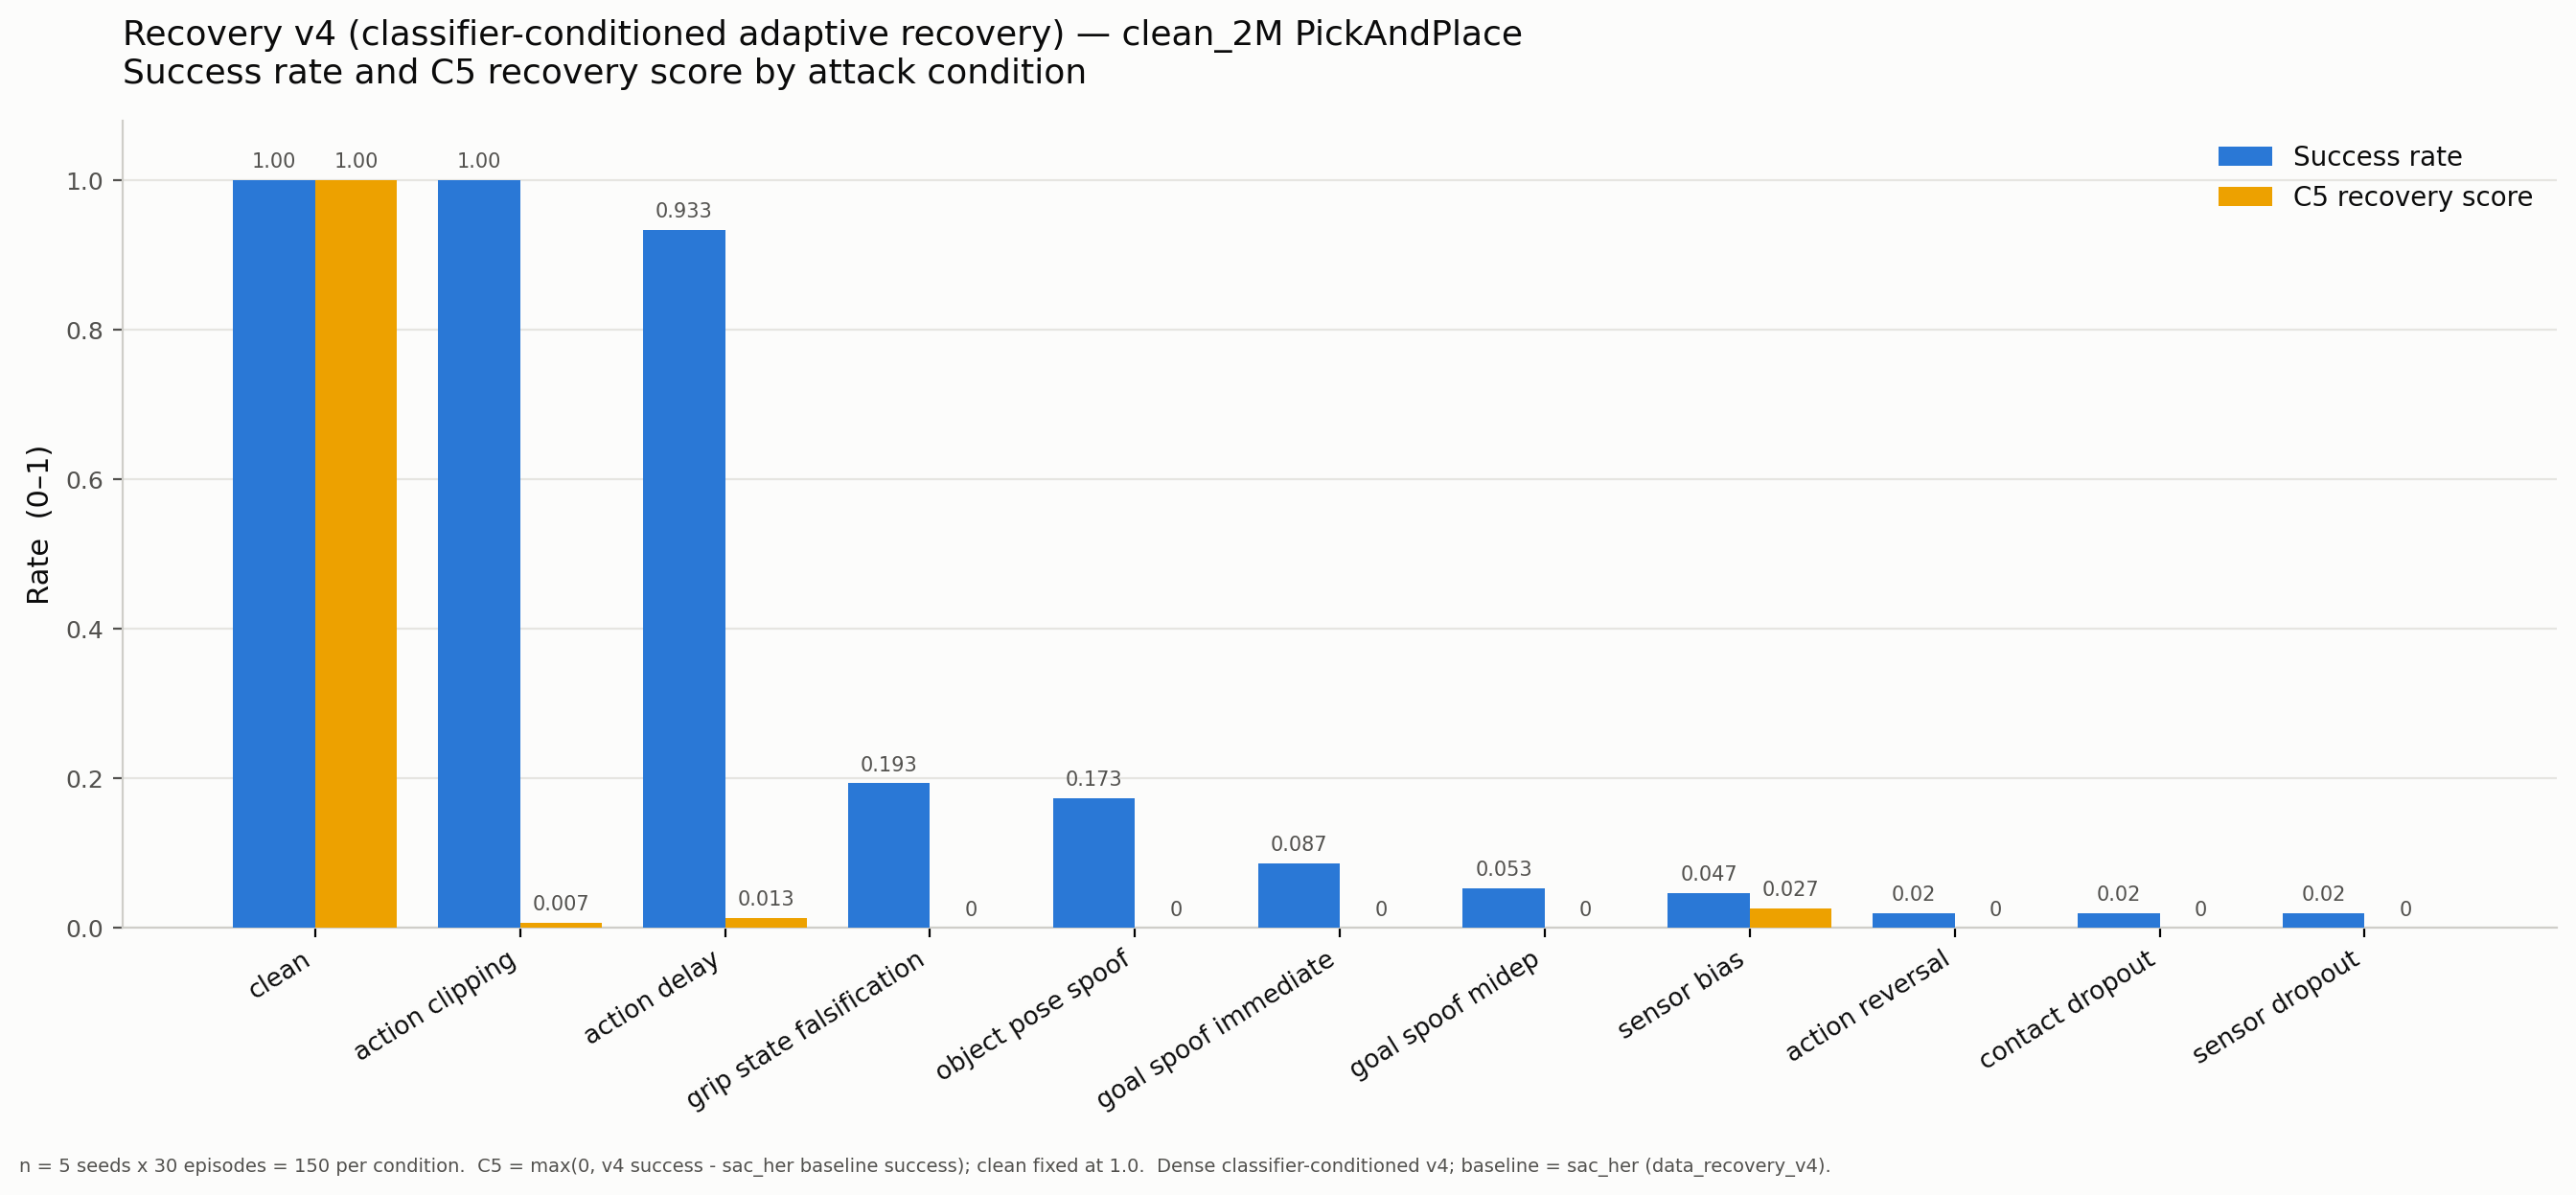
\includegraphics[width=\columnwidth]{paper_figures/recovery_v4_dense_sweep_by_condition.png}}
\caption{Recovery v4 (CCAR) on clean\_2M: per-condition success rate and $C_5$ recovery
lift. Recovery lift is nonzero only on the action-timing attacks; it is $0.000$ on goal
spoofing and grip falsification.}
\label{fig:v4_sweep}
\end{figure}

\begin{figure}[htbp]
\centerline{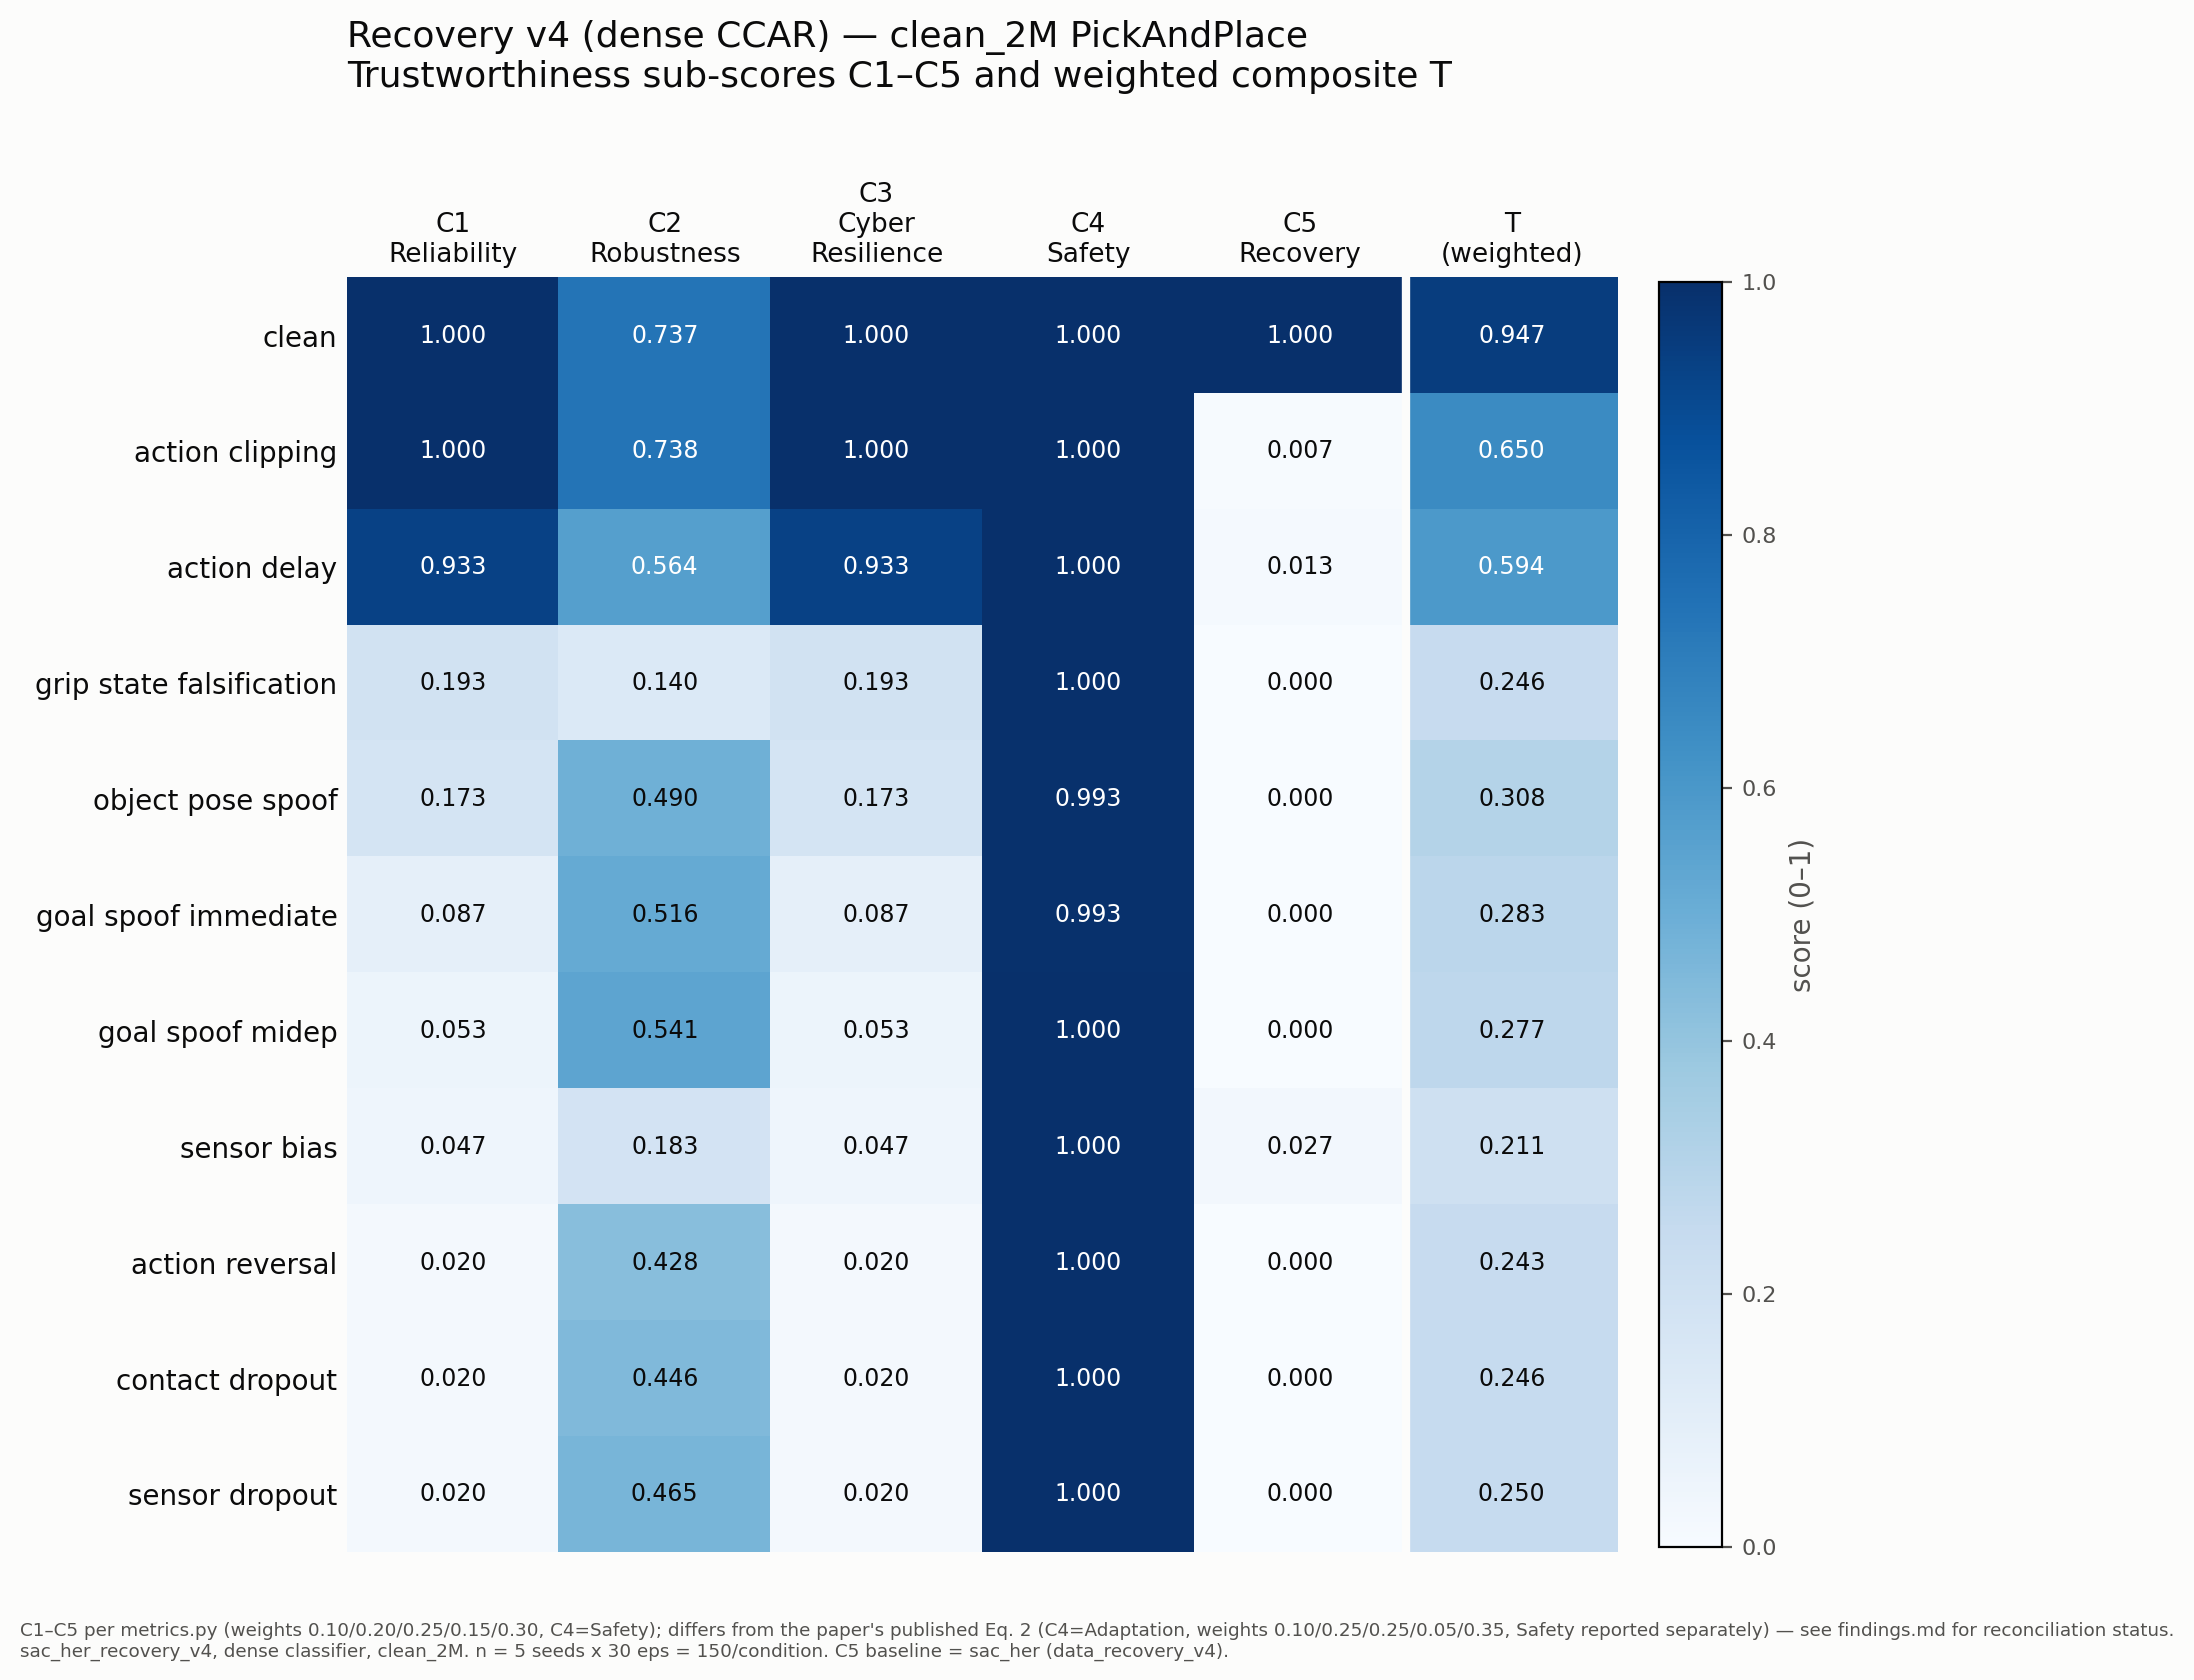
\includegraphics[width=\columnwidth]{paper_figures/recovery_v4_dense_trustworthiness_heatmap.png}}
\caption{Recovery v4 (CCAR) on clean\_2M: trustworthiness sub-scores $C_1$--$C_5$ and the
weighted composite $T$ across all eleven conditions, using the weights of
Eq.~\ref{eq:trustworthiness_score}.}
\label{fig:v4_heatmap}
\end{figure}

\subsection{Domain-Randomized Training Ablation}
\label{sec:randomized_ablation}

In addition to the clean-trained policy, we trained a second SAC+HER policy using an
\texttt{AttackRandomizationWrapper} that exposes the agent to attack conditions during
training with probability $1-p_{\mathrm{clean}}$, where $p_{\mathrm{clean}}=0.2$. This
domain-randomization approach is a natural robustness baseline, since exposing a policy
to perturbations during training is a standard strategy for closing the gap between
clean-task competence and attack resilience.

We evaluated this randomized policy at two training budgets, and the outcome is
budget-dependent (Table~\ref{tab:pnp_no_recovery}). At 500k steps the randomized policy
fails outright: $1.3\%$ clean success, near the floor across all conditions,
indistinguishable from the clean-trained 500k checkpoint and consistent with never
acquiring the grasp. At 2M steps it recovers partial competence: $44.7\%$ clean success
(final distance $0.188$~m, versus the clean-trained 2M policy's $100\%$ and $0.023$~m),
with comparable partial success under action clipping ($46.0\%$), action delay
($35.3\%$), and grip falsification ($34.0\%$). Additional training therefore does help
under randomization, but only partway and only at the larger budget; the randomized 2M
policy stays well below the clean-trained policy on every condition.

We read this as a scoped negative result at the 500k budget and a partial-competence
result at 2M, not a successful robustness/performance trade-off. Critically, the
randomized policy does not outperform the clean-trained policy on any individual attack
condition, which is the signature a successful trade-off would produce. With
$p_{\mathrm{clean}}=0.2$, $80\%$ of training episodes are conducted under attack, and
several of these directly corrupt the gripper action or object-position observation, the
two signals most critical to learning the grasp phase; we hypothesize that this starves
the multi-phase approach-grasp-lift-transport-release behavior of clean signal, so that
at 500k the base skill is not acquired at all and at 2M only partially. Retraining with
a substantially higher $p_{\mathrm{clean}}$, or a curriculum that establishes clean-task
competence before introducing attack exposure, is the natural next step and is left to
future work. Per-checkpoint success rates for all conditions are given in
Table~\ref{tab:pnp_no_recovery}.

\subsection{Trustworthiness Score Summary}

Table~\ref{tab:composite_scores} reports the composite trustworthiness score $T$
(Eq.~\ref{eq:trustworthiness_score}) and its sub-scores $C_1$--$C_5$ for SAC+HER
(clean\_2M) without recovery, computed by the evaluation pipeline's \texttt{metrics.py}
module via \texttt{build\_benchmark\_table.py} on the seed-fixed data. $C_2$ is
normalized dataset-relative over the SAC+HER (no-recovery) conditions.

\begin{table}[t]
\centering
\caption{Composite trustworthiness scores $C_1$--$C_5$ and $T$ for SAC+HER (clean\_2M),
FetchPickAndPlace-v4 ($n=150$ episodes per condition, no recovery). $C_5$ is $1.0$ for
clean by convention and $0.0$ for the no-recovery baseline rows; Recovery v4's $C_5$ lift
is reported in Section~\ref{sec:recovery_results}.}
\label{tab:composite_scores}
\begin{tabular}{lcccccc}
\toprule
Condition & $C_1$ & $C_2$ & $C_3$ & $C_4$ & $C_5$ & $T$ \\
\midrule
Clean                 & 1.000 & 0.879 & 1.000 & 1.000 & 1.000 & 0.976 \\
Sensor Dropout        & 0.020 & 0.525 & 0.020 & 1.000 & 0.000 & 0.262 \\
Sensor Bias           & 0.040 & 0.130 & 0.040 & 0.993 & 0.000 & 0.189 \\
Action Clipping       & 0.993 & 0.874 & 0.993 & 1.000 & 0.000 & 0.672 \\
Action Delay          & 0.920 & 0.773 & 0.920 & 1.000 & 0.000 & 0.627 \\
Action Reversal       & 0.020 & 0.500 & 0.020 & 1.000 & 0.000 & 0.257 \\
Goal Spoof (Imm.)     & 0.060 & 0.622 & 0.060 & 0.993 & 0.000 & 0.294 \\
Goal Spoof (Mid-ep)   & 0.093 & 0.676 & 0.093 & 1.000 & 0.000 & 0.318 \\
Object Pose Spoof     & 0.260 & 0.749 & 0.260 & 0.993 & 0.000 & 0.390 \\
Grip Falsification    & 0.207 & 0.182 & 0.207 & 0.993 & 0.000 & 0.258 \\
Contact Dropout       & 0.020 & 0.511 & 0.020 & 1.000 & 0.000 & 0.259 \\
\bottomrule
\end{tabular}
\end{table}

The scores separate cleanly into two bands. SAC+HER sustains reliable task completion
($T = 0.63$--$0.98$) under the clean condition and the two action-timing attacks it
rarely fails (action clipping, action delay); every other condition collapses
reliability toward the floor, pulling $T$ into the $0.19$--$0.39$ range even though
safety ($C_4$) stays near $1.0$ because the failing policy still moves without abnormal
actuator jerk. The lowest scores, sensor bias ($T=0.189$) and grip falsification
($T=0.258$), are driven jointly by near-zero reliability and low robustness ($C_2=0.130$
and $0.182$), distinguishing them from conditions like sensor dropout where the policy
fails the task but the object barely moves, keeping $C_2$ moderate.

These are the no-recovery baseline scores: $C_5$ is $1.0$ for clean by convention and
$0.0$ for every attacked SAC+HER row, since a base policy has no recovery lift over
itself. Recovery v4's per-condition $C_5$ lift on this same checkpoint is reported in
Section~\ref{sec:recovery_results}; it is nonzero only for the action-timing attacks, so
the composite gains from recovery are concentrated there.

We separately report a trajectory-progress \emph{adaptation} diagnostic
(Table~\ref{tab:adaptation_diagnostic}), which is computed but excluded from the weighted
composite (Section~\ref{sec:method}) because it is strongly collinear with reliability on
this task. The safety sub-score $C_4$ is a weighted composite term (Table~\ref{tab:composite_scores});
its jerk-based derivation is described in Section~\ref{sec:discussion}.

\begin{table}[t]
\centering
\caption{Diagnostic: trajectory-progress adaptation score
$\max(0,(d_{\mathrm{start}}-d_{\mathrm{final}})/(d_{\mathrm{start}}+\epsilon))$ (SAC+HER,
clean\_2M, no recovery). Reported separately; not a weighted term in the composite $T$
(Section~\ref{sec:method}).}
\label{tab:adaptation_diagnostic}
\begin{tabular}{lc}
\toprule
\textbf{Condition} & \textbf{Adaptation (mean $\pm$ std)} \\
\midrule
Clean               & $0.887 \pm 0.020$ \\
Sensor Dropout       & $0.000 \pm 0.000$ \\
Sensor Bias          & $0.015 \pm 0.011$ \\
Action Clipping      & $0.865 \pm 0.025$ \\
Action Delay         & $0.812 \pm 0.028$ \\
Action Reversal      & $0.000 \pm 0.000$ \\
Goal Spoof (Imm.)    & $0.525 \pm 0.051$ \\
Goal Spoof (Mid-ep)  & $0.538 \pm 0.065$ \\
Object Pose Spoof    & $0.653 \pm 0.076$ \\
Grip Falsification   & $0.224 \pm 0.066$ \\
Contact Dropout      & $0.000 \pm 0.000$ \\
\bottomrule
\end{tabular}
\end{table}

Adaptation tracks how far the object is moved toward the goal, independent of whether the
$0.05$~m success threshold is met. It is high where the policy succeeds or nearly
succeeds (clean $0.887$, action clipping $0.865$, action delay $0.812$) and exactly zero
where the object never moves (sensor dropout, action reversal, contact dropout),
confirming those are grasp-phase failures rather than near-misses. The goal-spoofing and
object-pose-spoofing conditions sit in between ($0.53$--$0.65$): the policy transports the
object a substantial distance toward a corrupted target but does not reach the true goal.
This diagnostic is strongly collinear with reliability, which is why it is reported here
rather than weighted into $T$.


% =============================================================================
\section{Discussion}
\label{sec:discussion}
% =============================================================================

\subsection{Policy-Dependent Attack Surfaces}

The central finding of TAIRO, consistent across both the FetchReach-v4 pilot and the
FetchPickAndPlace-v4 evaluation, is that adversarial vulnerability is not determined by
the attack type alone. Instead, attack effectiveness depends on the interaction between
the compromised channel and the policy architecture. SAC+HER depends heavily on the
policy-visible observation field when selecting motor commands, so attacks such as
sensor dropout and sensor bias are expected to degrade its performance substantially,
while the rule-based controller, which relies primarily on goal-space and
object-relative information, is expected to be comparatively insensitive to
proprioceptive corruption. This replicates only partially in our PickAndPlace results:
SAC+HER's own profile shows the same channel-dependent collapse (complete failure
under sensor dropout and sensor bias, full resilience under action clipping and delay;
Section~\ref{sec:results}), but we did not evaluate a rule-based controller on
PickAndPlace in this study, so the complementary claim, that a goal-space-reliant
controller remains robust to these same attacks, is untested at this task scale and
should not be assumed to hold without that baseline.

This result has an important implication for adversarial RL benchmarking. Robustness
scores should be interpreted as properties of policy--attack pairs rather than as
standalone properties of either the environment or the attack. For example, an
observation-space perturbation can be catastrophic for a learned policy that depends on
the full observation dictionary, but largely irrelevant to a controller that does not
use the corrupted field. Thus, benchmark results such as those reported in
Robust-Gymnasium~\cite{gu2025robustgymnasium} should be complemented with explicit
analysis of which policy inputs and control channels are actually used by the evaluated
agent.

\subsection{Recovery Depends on Detector--Attack Alignment}

The recovery experiments on the FetchReach-v4 pilot show that recovery is effective
only when the detector is aligned with the behavioral signature of the attack. The
initial v1 detector used general action divergence and increasing distance from the
goal as warning signs. However, this produced false positives on clean SAC+HER episodes
because healthy policies often generate large action changes during early convergence.
This failure shows that recovery detectors should not be calibrated only to generic
abnormality. They must instead target attack-specific signatures that distinguish
compromised execution from normal transient behavior.

Recovery v2 improves this alignment by monitoring sustained action-norm saturation.
Recovery v3 further improves the response by holding the fallback controller for
multiple steps after detection, allowing corrective behavior to accumulate over time.
The improvement from v2 to v3 on FetchReach-v4 demonstrates that recovery is not only a
detection problem; it is also a response-duration problem.

At the same time, the detector monitors action-space signals, while the attacks that
cause the most severe degradation, sensor dropout and goal spoofing, damage the
observation space instead. This is a structural mismatch, not simply a calibration gap:
a policy pursuing a corrupted goal or operating on zeroed observations can still
produce smooth, low-norm actions, so the detector may not fire even when the underlying
state is compromised. We treat this detection/damage mismatch as a research finding in
its own right, and one we expect to be more, not less, pronounced on
FetchPickAndPlace-v4, where object-pose spoofing and contact dropout corrupt
object-relative observation fields that are not reflected in action magnitude at all.
This suggests that future recovery systems should combine action-level signals with
goal-consistency checks, secure command authentication, and independent state or task
verification. To address this mismatch directly, we built a post-hoc failure-mode
classifier (Random Forest) over six behavioral labels (\texttt{success},
\texttt{never\_reached\_object}, \texttt{reached\_but\_failed\_grasp},
\texttt{grasped\_but\_dropped}, \texttt{spoofed\_goal}, and
\texttt{divergent\_transport}), trained on full-episode trajectory features rather than
attack-condition labels, so it distinguishes failure modes by behavior rather than by
which channel was attacked ($0.942$ accuracy, $0.816$ macro-F1). An online,
causal-feature version usable during execution is competitive with it ($0.948$ accuracy,
$0.839$ macro-F1 despite using only rolling, non-hindsight features), and it drives the
Recovery v4 trigger and expert-mixing weights (Section~\ref{sec:method}). This lets
recovery respond even when damage is confined to the observation space, where the
action-norm detector is blind, although Section~\ref{sec:recovery_results} shows the
resulting recovery is bounded by the classifier's early-episode reliability.

\subsection{Recoverability Varies Across Attack Classes}

The FetchReach-v4 pilot also shows that attacks differ not only in severity but also in
recoverability. Sensor dropout is severe for SAC+HER when unrecovered, but is also
highly recoverable when a trusted fallback controller has access to reliable goal and
end-effector information. By contrast, action reversal remains difficult to recover
under the current design, because the adversary directly inverts every issued command,
including commands produced by the fallback controller. This highlights a fundamental
difference between observation-channel failures and action-channel hijacks:
observation attacks may be mitigated by a trusted fallback perception or state
estimation, while full action-channel compromise requires secure actuation, command
authentication, or a lower-level safety controller outside the compromised channel.
Recoverability of the manipulation-specific attacks is measured directly on PickAndPlace
by Recovery v4 (Section~\ref{sec:recovery_results}): object pose spoofing, grip
falsification, and contact dropout all receive $0.000$ recovery lift, consistent with
their damage residing in the observation or grasp-integrity channel rather than in
recoverable action timing. Object pose spoofing has the highest no-recovery partial
success of the three ($26.0\pm3.3\%$, in the range of goal spoofing), yet Recovery v4
does not improve it, underscoring that partial no-recovery success and recoverability are
distinct properties: the object is moved toward a corrupted target, and no action-timing
correction redirects it to the true goal.

\subsection{Limitations}

\textbf{Oracle recovery privilege.}
The current recovery controller uses the simulator's raw, unattacked state when
re-anchoring after detection. This design is useful for estimating the upper-bound value
of recovery-aware control, but it is not directly deployable. A physical robot would
need an independent, trusted sensing channel, a redundant state estimator, an external
verification module, or a secure goal-authentication mechanism to provide the same
information without relying on simulator privilege. This gap is scoped out of the
current work and flagged specifically for the planned Habitat/Isaac Sim transition,
where a robot could no longer be assumed to have direct access to ground-truth state.

\textbf{Attack magnitude calibration.}
Several attack magnitude constants, including sensor bias, action clipping, and the
goal-spoofing offsets, were carried over from the FetchReach-v4 pilot or set
provisionally by construction (matched to a shared offset scale across attacks) rather
than independently derived from FetchPickAndPlace-v4's observation distributions. In
particular, the sensor-bias offset of $\pm 0.10$ is disproportionately large relative to
the physical range of the gripper finger-width observation dimensions (approximately
0--0.05~m), representing roughly twice their full physical range rather than a
proportionate perturbation. Unlike the safety-score threshold discussed below, these
constants set the strength of an injected perturbation that is by definition absent in
clean episodes, so there is no clean-condition reference distribution to calibrate
against in the way the safety threshold was calibrated against clean-episode jerk. We
therefore report these magnitudes as provisional-by-construction and flag this as a
limitation rather than retrofitting a post-hoc justification; we do not expect it to
change the headline attack-vulnerability findings. An empirical magnitude sweep (e.g.,
testing offsets of 0.05, 0.10, and 0.20 against clean-episode outcome degradation to
confirm the chosen magnitude is neither negligible nor uniformly catastrophic) is a
natural next step and is left to future work.

\textbf{Safety sub-score (C4).}
An earlier version of the trustworthiness scoring module's safety-related component
computed a per-step action-norm safety-violation rate using a single threshold
calibrated for FetchReach-v4's three-dimensional action space. FetchPickAndPlace-v4's
action space adds a fourth (gripper) dimension, which raised the geometric action-norm
ceiling and caused routine gripper actuation to register as unsafe under the original
threshold, producing an inverted signal in which clean execution scored lower than an
artificially action-clipped condition. We resolved this with a structural redesign
rather than a simple threshold adjustment: the safety metric now splits arm and gripper
actuation into separate channels, computing a jerk-based (step-to-step action change)
violation signal for each, OR-fused into a single per-step flag. Each channel's
threshold is calibrated as a multiplier applied to the maximum observed jerk across
clean-condition episodes, not a percentile of the clean distribution. Verified against
150 clean-condition episodes, this redesigned metric produces zero safety violations
and zero false positives, correcting the inverted signal. This safety sub-component
($C_4$, \texttt{safety\_score}) is one of the five weighted terms in the composite score
(Eq.~\ref{eq:trustworthiness_score}); the trajectory-progress adaptation quantity that
occupied the fourth slot in earlier drafts is now reported as a standalone diagnostic
(Table~\ref{tab:adaptation_diagnostic}) instead, as it is strongly collinear with
reliability on this task.

\textbf{Single-seed training scope.}
Evaluation-seed variance is characterized throughout this work: each policy checkpoint
is evaluated across five random seeds (Section~\ref{sec:eval}), and reported statistics
reflect variation across those evaluation seeds. However, each policy checkpoint
(\texttt{clean\_500k}, \texttt{clean\_2M}, \texttt{randomized\_500k},
\texttt{randomized\_2M}) was itself trained from a single random initialization; we did
not train multiple independent seeds per checkpoint. Training-run-to-training-run
variance, i.e., whether a differently-initialized SAC+HER run would learn the same
clean-task competence or exhibit the same vulnerability profile, is therefore not
captured by our reported statistics. We leave multi-seed training as future work.

\textbf{Recovery scope and ceiling.}
Recovery v4 (CCAR) is evaluated on the clean-trained 2M checkpoint only; the other three
checkpoints lack a non-degenerate clean-condition failure-probability distribution to
calibrate the trigger, and the threshold-based v1--v3 controllers are validated only on
the FetchReach-v4 pilot (Appendix~\ref{app:fetchreach}). On PickAndPlace, Recovery v4
recovers the action-timing attacks but produces zero recovery lift on the observation-
and goal-channel attacks (Section~\ref{sec:recovery_results}). Retraining the online
classifier on dense every-step features did not raise this ceiling, which we trace to
intrinsic early-episode low information rather than to training coverage: in the first
steps of an episode the trajectory has not yet diverged enough for the classifier to
identify the failure mode, so the blend weight cannot rise in time to redirect an
observation- or goal-corrupted rollout. A stronger early-episode detector, or a redundant
trusted sensing channel, would be required to lift it. This is a concrete instance of the
broader principle that recovery quality is bounded by detector quality.

\textbf{Domain-randomized training outcome.}
As shown in Section~\ref{sec:randomized_ablation}, our attack-randomization curriculum
failed to learn the grasp phase at the 500k budget and recovered it only partially at 2M
($44.7\%$ clean success, far below the clean-trained policy). We report this as a
scoped negative-to-partial result rather than a completed robustness comparison, since
the randomized policy never outperforms the clean-trained policy on any condition; a
viable randomized-training baseline would require a substantially higher clean-episode
fraction or a staged curriculum, which we leave to future work.

\textbf{Limited simulation fidelity.}
FetchPickAndPlace-v4 is a MuJoCo-based manipulation task with idealized contact
dynamics and full state observability. This makes it useful for isolating the effects
of observation, goal, and action attacks in a controlled setting, but it does not
capture many challenges of real robotic systems, including visual perception errors,
object occlusion beyond what is modeled, deformable environments, or long-horizon
planning. Results may therefore change when TAIRO is migrated to more complex
environments such as Habitat-based home simulation or Isaac Sim.

\textbf{Incomplete attack coverage.}
TAIRO currently evaluates eleven attack conditions across observation, goal, action, and
manipulation-specific channels. It does not yet include Gaussian sensor noise, action
scaling, reward tampering, adversarial visual perturbations, localization attacks, or
multi-channel coordinated attacks. These attacks are important future extensions,
especially for higher-fidelity embodied-AI environments.

\textbf{Physical robot deployment.}
All results in this paper are obtained in MuJoCo simulation. We have acquired and
powered on a JetCobot physical manipulator as a candidate platform for a future
sim-to-real extension of TAIRO, but have not yet attempted to transfer the trained
SAC+HER policy to it. This transfer is nontrivial: our policy was trained entirely in
Gymnasium-Robotics simulation, and bridging to physical hardware would require
addressing differences in kinematics, perception (the simulator provides ground-truth
object pose, which a physical system would need to estimate), and control-loop timing.
We treat physical deployment as a multi-week future effort rather than an active
component of the current work.

\subsection{Toward Higher-Fidelity Simulation}

TAIRO is designed as a staged framework rather than a single-task benchmark. The first
stage used FetchReach-v4 to isolate core attack and recovery mechanisms in a controlled
goal-conditioned reaching environment (Appendix~\ref{app:fetchreach}). The current stage
uses FetchPickAndPlace-v4, where contact dynamics and grasp stability introduce the
manipulation-specific failure modes evaluated in this paper. The next stage will extend
the framework to higher-fidelity embodied-AI simulation environments such as
Habitat~\cite{puig2023habitat3} and Isaac Sim~\cite{nvidia2026isaacsim}, which make it
possible to evaluate whether the same attack taxonomy transfers to visually grounded
navigation, household robotics, and more realistic physics. We had considered a
world-model-based integration using Cosmos 3~\cite{agarwal2026cosmos3} as part of this
roadmap, which could in principle support diverse synthetic scenarios and stress
testing under environment variation; we do not pursue this in the current work due to
compute constraints, and leave it as a longer-term direction contingent on available
resources rather than a near-term milestone.

The key long-term research question is the fidelity gap: whether attacks and recovery
strategies that appear effective in lower-fidelity simulation remain effective as
perception, physics, and task complexity increase. Measuring this gap systematically,
first from FetchReach-v4 to FetchPickAndPlace-v4 and subsequently to Habitat and Isaac
Sim, is one of TAIRO's main future directions. By tracking how vulnerability profiles
change across this progression, TAIRO can provide a principled path toward
recovery-aware trustworthiness evaluation for real-world robotic systems.


% =============================================================================
\section{Conclusion}
\label{sec:conclusion}
% =============================================================================

We presented TAIRO, a recovery-aware trustworthiness evaluation framework for robotic
control policies under adversarial cybersecurity perturbations. Using FetchPickAndPlace-v4
as a contact-rich, sparse-reward manipulation benchmark, building on an initial
validation pilot on the lower-dimensional FetchReach-v4 task, TAIRO evaluates how
learned policies behave under observation-space, goal-space, action-space, and
manipulation-specific attacks, and whether online recovery can improve task outcomes
during execution.

Our results, together with the FetchReach-v4 pilot, support several main findings.
First, adversarial vulnerability is policy- and attack-surface-dependent: SAC+HER's
own channel-dependent vulnerability profile replicates as task complexity increases
from reaching to grasping and transport, though the complementary cross-architecture
claim (that a rule-based controller remains robust to the same attacks) is untested at
the PickAndPlace scale. Second, HER is a load-bearing component for sparse-reward
manipulation, established in the FetchReach-v4 pilot; this ablation was not repeated on
FetchPickAndPlace-v4 and remains a FetchReach-only finding carried forward as a design
decision. Third, recovery effectiveness depends on detector--attack alignment, and the
action-space detector's blindness to observation-space damage is a structural
limitation rather than a calibration artifact; this motivated the classifier-conditioned
Recovery v4 controller, which on PickAndPlace recovers the action-timing attacks but
leaves observation- and goal-channel damage unrecovered, a ceiling we trace to the
online classifier's early-episode reliability rather than to its training density. Fourth, trustworthiness scoring should be outcome-referenced,
so that recovery is credited only when it improves task success rather than merely
triggering frequently; this principle is unaffected by the PickAndPlace extension.
Fifth, robustness-oriented training strategies such as domain randomization are not
automatically beneficial: our attack-randomization curriculum failed to learn the base
grasping skill at the 500k budget and acquired it only partially at 2M ($44.7\%$ clean
success, well below the clean-trained policy), underscoring the need for sufficient
clean-task signal during training and confirming, rather than merely proposing, the
migration risk we anticipated when scaling beyond FetchReach-v4.

TAIRO provides a modular foundation for future recovery-aware robotics evaluation. Its
attack wrappers, policy interface, recovery controller, and trustworthiness scoring
module can be extended beyond FetchPickAndPlace-v4 to more complex manipulation and
embodied-AI settings. Future work will migrate the framework to Habitat and Isaac Sim
to study how vulnerability and recovery behavior change as task complexity, perception
fidelity, and physical realism increase. This fidelity-gap analysis is the next step toward a trustworthy
evaluation of robotic systems before deployment in safety-critical homes, hospitals,
and elder-care environments.



\section*{Acknowledgment}
This work was supported by the National Science Foundation Research Experiences for Undergraduates (NSF REU) program, Summer 2026, under NSF Grant No. CNS-2349236. Computational resources were provided by the University of Missouri--Kansas City.


\appendix
\section{FetchReach-v4 Pilot Study}
\label{app:fetchreach}

Prior to scaling TAIRO to FetchPickAndPlace-v4, we validated the framework on
FetchReach-v4, a lower-dimensional goal-conditioned reaching task with a 50-step
episode budget and an eight-condition attack taxonomy (the six attacks shared with
Section~\ref{sec:method}, excluding the three manipulation-specific attacks introduced
for PickAndPlace). Table~\ref{tab:fetchreach_pilot} summarizes SAC+HER performance
without recovery and under Recovery v3.

\begin{table}[htbp]
\caption{FetchReach-v4 Pilot: SAC+HER Success Rate (\%)}
\label{tab:fetchreach_pilot}
\begin{center}
\begin{tabular}{lcc}
\toprule
\textbf{Execution Condition} & \textbf{No Recovery} & \textbf{Recovery v3} \\
\midrule
Clean                   & 100 & 100 \\
Sensor Dropout          &   0 &  83 \\
Sensor Bias             &   9 &  20 \\
Goal Spoof (Immediate)  &   5 &   8 \\
Goal Spoof (Mid-Ep.)    &   9 &   7 \\
Action Clipping         & 100 & 100 \\
Action Delay            & 100 & 100 \\
Action Reversal         &   0 &   0 \\
\bottomrule
\end{tabular}
\end{center}
\end{table}

Two findings from this pilot directly shaped the FetchPickAndPlace-v4 study. First,
plain SAC without HER achieved 0\% success across all conditions, including clean
execution, confirming that HER is necessary rather than merely beneficial for
sparse-reward manipulation under our training budget; we therefore did not repeat this
ablation for FetchPickAndPlace-v4. Second, the recovery controller's iterative design,
from an uncalibrated v1 detector that false-triggered on 100\% of clean episodes, to
the action-norm-saturation-based v2, to the sustained-intervention v3, was developed
and validated in this lower-dimensional setting before being carried forward to
FetchPickAndPlace-v4. As in the main study, recovery provided the largest benefit under
sensor dropout, and action reversal remained unrecoverable within the fixed episode
budget, establishing the detector--attack alignment and full-hijack limitations
discussed in Section~\ref{sec:discussion}.

Also notable: the rule-based controller in this pilot maintained 100\% success under
sensor dropout, sensor bias, and goal spoofing, since it relies primarily on
goal-space and end-effector position rather than the corrupted proprioceptive
observation field. This result should be interpreted as an oracle-style upper bound on
what a trusted fallback mechanism could achieve given reliable goal and end-effector
information, not as evidence that the rule-based controller is robust in a general
sense.


\bibliographystyle{IEEEtran}
\bibliography{references}


\end{document}